\section{Overview}

\begin{defn}[Voter Model] \cite{Liggett2002}
Let $G = (V,E)$ be a graph with finite or countably infinite vertices (such as $\Z^d$) and $P$ be the transition probability matrix for a Markov chain on $G$.
Then $S = \{0,1\}^{V}$ is the state space for voter model which is a continuous-time Markov chain.
For $\eta \in S$ denote $\eta(x)$ as the value of the node $x \in V$ in the configuration $\eta$.
Let $\eta_x$ be the configuration obtained by changing the value of $\eta$ at the site $x$. That is,
$$
\eta_x(y) = \begin{cases}
    \eta(y) & x \not = y\\
    1 - \eta(y) & x = y
\end{cases}
$$

If $S$ is a finite, e.g. a subset of $\{0,1\}^{\Z^d}$, then $\eta$ transitions to $\eta_x$ at a rate of
$$
q(\eta, \eta_x) = \sum_{y : \eta(y) \not = \eta(x)} P(x,y)
$$
Thus, for any $\eta, \delta \in S$ that differ by more than one sites,
$$
q(\eta, \delta) = 0
$$
and $\eta \in S$ transitions to $\delta \in S$ with probability
$$
P^\eta(\eta_t = \delta) = q(\eta, \delta) t + o(t)
$$
as $t \downarrow 0$.

If $S$ is infinite then it is more technical to define the process. In this thesis we focus on finite $S$ but the reader can find descriptions of the infinite case in \cite{Liggett1999} or \cite{Liggett2002}.

In general we assume that on $Z^d$ then $P(x,y) = P(0, x - y)$
where $P(x- y) = \frac{1}{2d}$ if $x$ and $y$ are adjacent and $P(x-y) = 0$ otherwise.
\end{defn}

\begin{defn} \cite{Liggett1999}
If $\mu, \nu$ are probability measures on $\{0,1\}^S$ then $\nu \leq \mu$ if
$$
\int f~d\nu \leq \int f~d\mu
$$
for all bounded increasing functions on $\{0,1\}^S$
\end{defn}

\begin{theorem}
The transition rates have the following properties:
\begin{enumerate}
    \item $q(\eta, \eta_x) = 0$ for each $x \in \Z^d$ if $\eta \equiv 0$ or $\eta \equiv 1$
    \item $q(\eta, \eta_x) = q(\zeta, \zeta_x)$ for every $x \in \Z^d$ if $\eta(y) + \zeta(y) = 1$ for all $y \in \Z^d$. That is, the dynamics of the system are not changed by interchanging 1 and 0.
    \item (Monotonicity) $q(\eta, \eta_x) \leq q(\zeta, \zeta_x)$ if $\eta \leq \zeta$ and $\eta(x) = \zeta(x) = 0$
    \item $q(\eta, \eta_x)$ is invariant under shifts in $\Z^d$.
\end{enumerate}
\end{theorem}

In Figure \ref{fig:voter_sim_1d_torus.png} we show one realization from a simulation of the voter model with periodic boundaries on length 300 subset of $\Z$.
In Figure \ref{fig:voter_sim_2d_torus.png} we show one realization from a simulation of the voter model with periodic boundaries on a $100 \times 100$ grid.

\begin{figure}[H]
  \centering
    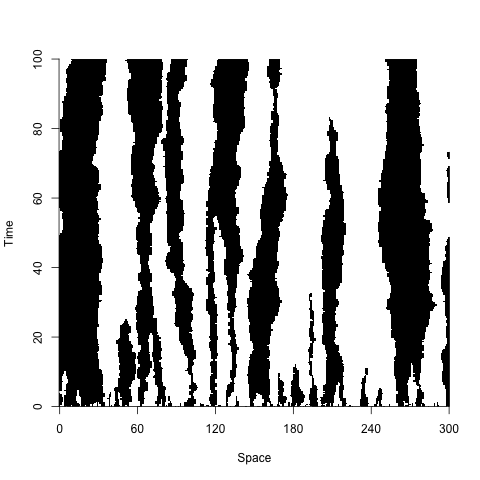
\includegraphics[width=.80\textwidth]{figures/voter_simulation_1d_300.png}
   \caption{Simulation for voter model with periodic boundary conditions on length 300 subset of $\Z$}
  \label{fig:voter_sim_1d_torus.png}
\end{figure}

\begin{figure}[H]
  \centering
    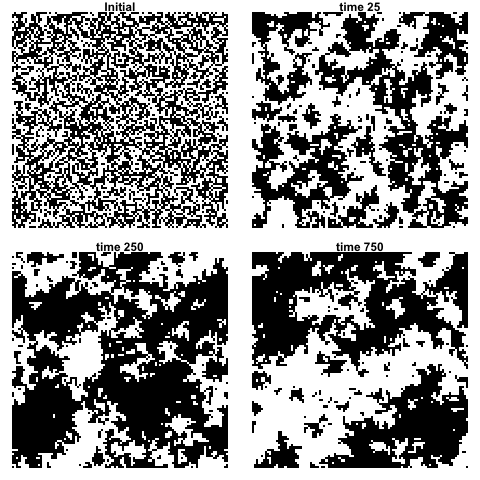
\includegraphics[width=.80\textwidth]{figures/voter_simulation_torus_100.png}
   \caption{Simulation for voter model with periodic boundary conditions on $100 \times 100$ grid.}
  \label{fig:voter_sim_2d_torus.png}
\end{figure}

\section{Voter Model Dual Process}

Assume that we have a voter model on $\Z^d$.
This description of the dual process for the voter model is a summary of \cite{Liggett1999}.
We introduce the graphical representation as follows: For every $x \in \Z^d$ there are $d$ corresponding Poisson processes, denoted $\{N_{x,x'}(t), t \geq 0\}$ for each $|x - x'| = 1$, with rate $\frac{1}{2d}$.
This is shown in Figure \ref{fig:voter_model_dual} for one dimension.
The arrows from $x$ to $y$ depicts the points of the Poisson process $\{N_{x,y}(t), t \geq 0\}$ which represent when $y$ changes its value to the value at site $x$.
Then by Poisson superposition (Theorem \ref{thm:poisson_super}) we can combine all the $d$ Poisson processes emanating from each site $x$ into one Poisson process with rate $1$.
The site $x$ waits exponential time with rate $1$ and then selects one of its $\frac{1}{2d}$ neighbors to conform to the same value as $x$.
Then the voter model with initial state $\eta_0$ is denoted by $\{\eta_t^{\eta_0}\}$ where $\eta_t^{\eta_0}(x)$ is the value of the voter model at site $x$.
This corresponds to sliding down the graphical representation, following arrows backwards until we reach the value at $\eta_0$.

Now we can define the dual process.
For each $x \in \Z^d$ at a time $t \geq 0$,
denote $A_{x,t}(s) \in \Z^d$ for $0 \leq s \leq t$ as the location on $Z^d$ as we follow the path downwards and moving in the reverse direction on the arrows. This is illustrated in the right figure of Figure \ref{fig:voter_model_dual}.
The process is $\{A_{x,t}(s) : 0 \leq s \leq t\}$, which is a continuous time random walk with rate $1$ jumps with probability $\frac{1}{2d}$ to each of its neighbors.
For 2 sites $x, y \in \Z^d$ we have
$\{A_{x,t}(s) : 0 \leq s \leq t\}$ and $\{A_{y,t}(s) : 0 \leq s \leq t\}$ that are independent until they meet.
The difference between two random walks is also a random walk.
Thus, $\{A_{x,t}(s) - A_{y,t}(s) : 0 \leq s \leq t, x,y \in \Z^d\}$ is a random walk with rate $2$ that moves to one of its $2d$ neighbors.
Once it hits 0 then it will remain 0.

We will need this important fact about random walks

\begin{theorem}[Random walk recurrent/transient] \label{thm:rw_recurrent}
Assume that $\{X_t\}$ is a random walk on $\Z^d$.
If $d = 1,2$ then it is recurrent.
If $d \geq 3$ then it is transient.
\end{theorem}

\begin{theorem}[\cite{Liggett1999}]
For $d = 1,2$ the voter model on $\Z^d$ with any initial configuration then
$$
\lim_{t \to \infty} P(\eta_t(x) \not = \eta_t(y)) = 0
$$
for all $x,y \in \Z^d$.
This behavior is called \textbf{clustering}.
\end{theorem}

\begin{proof}
Take $x, y \in \Z^d$ and let $\{A_{x,t}(s) : 0 \leq s \leq t, x \in \Z^d\}$ and $\{A_{y,t}(s) : 0 \leq s \leq t\}$ be the random walks for a fixed time $t$.
Once $A_{x,t}(\tau) = A_{y,t}(\tau)$ for some $\tau \in [0, t]$ then the voter model process must agree, e.g. $\eta_t(x) = \eta_t(y)$.
Thus
\begin{align*}
P(\eta_t(x) \not = \eta_t(y)) \leq P(A_{x,t}(s) - A_{y,t}(s) \not = 0 : 0 \leq s \leq t)
\end{align*}

% Then $\eta_t(x) = \eta_t(y)$ can happen for one of two reasons
% \begin{itemize}
%     \item $A_{x,t}(s) = A_{y,t}(s)$ and $s < \tau$,
%     \item $s > \tau$
% \end{itemize}

Taking the limit as $t \to \infty$ the RHS goes to 0 by Theorem \ref{thm:rw_recurrent} since $\{A_{x,t}(s) - A_{y,t}(s) : 0 \leq s \leq t\}$ is recurrent for $d = 1,2$.
\end{proof}

\begin{figure}[H]
  \centering
    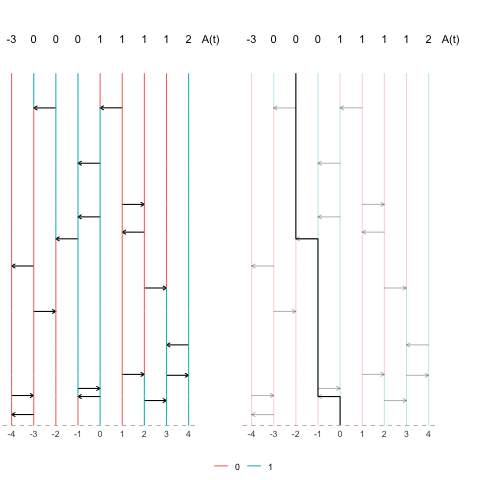
\includegraphics[width=1\textwidth]{figures/voter_model_dual.png}
   \caption{Voter model process with one particular path highlighted to show how $A(t)$ is computed for the site $-2$.}
  \label{fig:voter_model_dual}
\end{figure}

\section{Finite Voter Model}
We will now look at the time for voter model on a finite cycle and complete graph to reach the configuration of all 1's or all 0's.
In general there are $2^n$ configurations for the these graph but many of these have the same rates due to rotations and the property that interchanging 1's and 0's are equivalent.
That is, if $\eta$ is a configuration then $1 - \eta$ should be in the same equivalence class.

In the complete graph each node in a configuration is connected to all of the others, we can project a configuration $\eta$ to the minimum number of 1's in $\eta$ and $1 - \eta$.
$$
\eta \mapsto \min\left(|\{x : \eta(x) = 1\}|, |\{x : \eta(x) = 0\}|  \right)
$$
We will have $\lfloor n/2 \rfloor + 1$ new projected states for a voter model on a complete graph with $n$ nodes which will be a Markov chain
by Theorem \ref{thm:mc_projection}.

For all of the following models we will be using the following transition probability matrix
$$
P(x,y) = P(y,x) = \frac{1}{\deg(x)}
$$
Where $\deg(x)$ is the degree of the node $x$.
So in the case of the cycle, $P(x,y) = 1/2$, and the complete graph with $n$ nodes $P(x,y) = 1/(n - 1)$.

Denote $C_i$ as a complete graph with $i$ vertices.
In the complete graph each vertex has an edge between all $i - 1$ other vertices in the graph.

\begin{figure}[H]
  \centering
    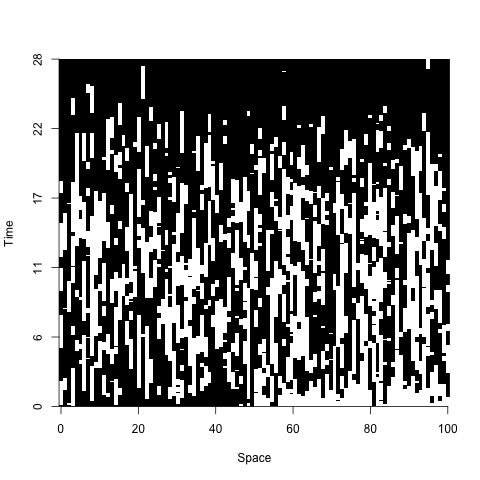
\includegraphics[width=.80\textwidth]{figures/voter_simulation_1d_complete_split_100.png}
   \caption{Simulation for voter model on a complete graph with 100 nodes. The initial configuration is split with half 1's and half 0's.}
  \label{fig:voter_sim_1d_complete.png}
\end{figure}

\subsection{Two node complete/cycle}
A complete graph (or a cycle) with $n = 2$ nodes has two projected states, $\{0,1\}$.
Assuming that we initialize the voter model to state 1, then we will just wait exponential time with rate 1 before going to the absorbing state 0.

\subsection{Three node complete/cycle}
A complete graph (or a cycle) with $n = 3$ nodes has two projected states, $\{0,1\}$.
Similarly to the two node case, if we initialize the voter model to state 1, then we will just wait exponential time with rate 1 before going to the absorbing state 0.

\subsection{Four node complete voter model \texorpdfstring{$C_4$}{VC4}}
We will now see that when we move to $n = 4$, we will get a more interesting distribution for the absorption time.
The state space in the projected four node voter model is $\{0,1,2\}$.
When we are in state 2, then all nodes can switch from 1 to 0 or 0 to 1.
Each of these switch at a rate of $2 \cdot 1/(4 - 1) = 2/3$ since they are connected to 2 other nodes with the opposite value.
Thus, the rate from $2 \to 1$ is $8/3$.
Similarly reasoning leads us to the rates in the form of the infinitesimal generator matrix
% 2 -> 1 rate 2 * 1/(4 - 1) * 2 = 4/3 is
$$
Q_{C_4} = \begin{blockarray}{cccc}
    & 2 & 1 & 0\\
    \begin{block}{c|ccc}
        \cline{2-4}
        2 & -\frac{8}{3} & \frac{8}{3} & 0 \\
        1 & 1 & -2 & 1\\
        0 & 0 & 0 & 0\\
    \end{block}
\end{blockarray}
$$
Let
\begin{align*}
    \mathbf{S} &= \begin{bmatrix}
    -\frac{8}{3} & \frac{8}{3}\\
    1 & -2\\
    \end{bmatrix}\\
    \mathbf{S}_0 &= (0, 1)^T
\end{align*}
Then the eigenvalues are determined by the characteristic polynomial
$$
(8/3 + m)(2 + m) - 8/3 = m^2 + \frac{14}{3} m + \frac{8}{3}
$$
which has roots of $m_1 = -4$ and $m_2 = - \frac{2}{3}$.
So the eigenvalues of $xS$ are $\lambda_1 = -4x$ and $\lambda_2 =  - \frac{2}{3} x$.
These eigenvalue have corresponding eigenvectors of $v_1 = (-2, 1)$ and $v_2 = (4/3, 1)$.
Let
$$
U = \begin{bmatrix}
    -2 & 4/3\\
    1 & 1
\end{bmatrix}
$$
thus
$$
U^{-1} = \frac{1}{10} \begin{bmatrix}
    -3 & 4\\
    3 & 6
\end{bmatrix}
$$
So the diagonalization of $S$ is given as
$$
\mathbf{S} = \begin{bmatrix}
    -2 & 4/3\\
    1 & 1
\end{bmatrix} \operatorname{diag}(-4x, - \frac{2}{3} x)
\frac{1}{10} \begin{bmatrix}
    -3 & 4\\
    3 & 6
\end{bmatrix}
$$
By Theorem \ref{thm:phase-type-pdf-cdf}, where $(\alpha_2, \alpha_1)$ is the probability of starting in state 2 and 1 respectively, we have the density of the absorption time $\tau_{C_4}$ is given as
\begin{align*}
    f_{C_4}(x) &= (\alpha_2, \alpha_1) \exp(x\mathbf{S}) \mathbf{S}_0\\
    &= \frac{1}{10} (\alpha_2, \alpha_1) \begin{bmatrix}
    -2 & 4/3\\
    1 & 1
\end{bmatrix}
\begin{bmatrix}
\exp(-4x) & 0\\
0 & \exp(- \frac{2}{3} x))
\end{bmatrix}
\begin{bmatrix}
    -3 & 4\\
    3 & 6
\end{bmatrix}
(0,1)^T\\
&= \frac{1}{10} (\alpha_2, \alpha_1)
\begin{bmatrix}
-2 \exp(-4x) & \frac{4}{3} \exp(-\frac{2}{3} x)\\
\exp(-4x) & \exp(- \frac{2}{3} x))
\end{bmatrix}
\begin{bmatrix}
    4\\
    6
\end{bmatrix}\\
&= \frac{1}{5} (\alpha_2, \alpha_1)
\begin{bmatrix}
-4 \exp(-4x) + 4 \exp(-\frac{2}{3} x)\\
2 \exp(-4x) + 3 \exp(-\frac{2}{3} x)
\end{bmatrix}\\
&= \frac{1}{5} \left[ \alpha_2 \left( -4 \exp(-4x) + 4 \exp\left(-\frac{2}{3} x\right) \right) + \alpha_1 \left( 2 \exp(-4x) + 3 \exp\left(-\frac{2}{3} x\right) \right) \right]\\
&= \frac{1}{5} \left[ (-4 \alpha_2 + 2 \alpha_1) \exp(-4x) + (4 \alpha_2 + 3 \alpha_1) \exp\left(-\frac{2}{3} x\right)\right]
\end{align*}

In Figure \ref{fig:voter_density_c4} we plot the density function for $\tau_{C_4}$ for varying $\boldsymbol{\alpha} = (\alpha_2, \alpha_1)$ values.
The expected value of $\tau_{C_4}$ is given by Theorem \ref{thm:phase-moments}
\begin{align*}
    E[\tau_{C_4}] &= -1 (\alpha_2, \alpha_1) \mathbf{S}^{-1} (1, 1)^T\\
    &= \frac{1}{8} (\alpha_2, \alpha_1) \begin{bmatrix}
    6 & 8\\
    3 & 8
    \end{bmatrix} (1,1)^T\\
    &= \frac{7}{4} \alpha_2 + \frac{11}{8} \alpha_1
\end{align*}
So when deterministically starting at state 2, we have that the expected value of the waiting time is $\frac{7}{4}$.

\begin{figure}[H]
  \centering
    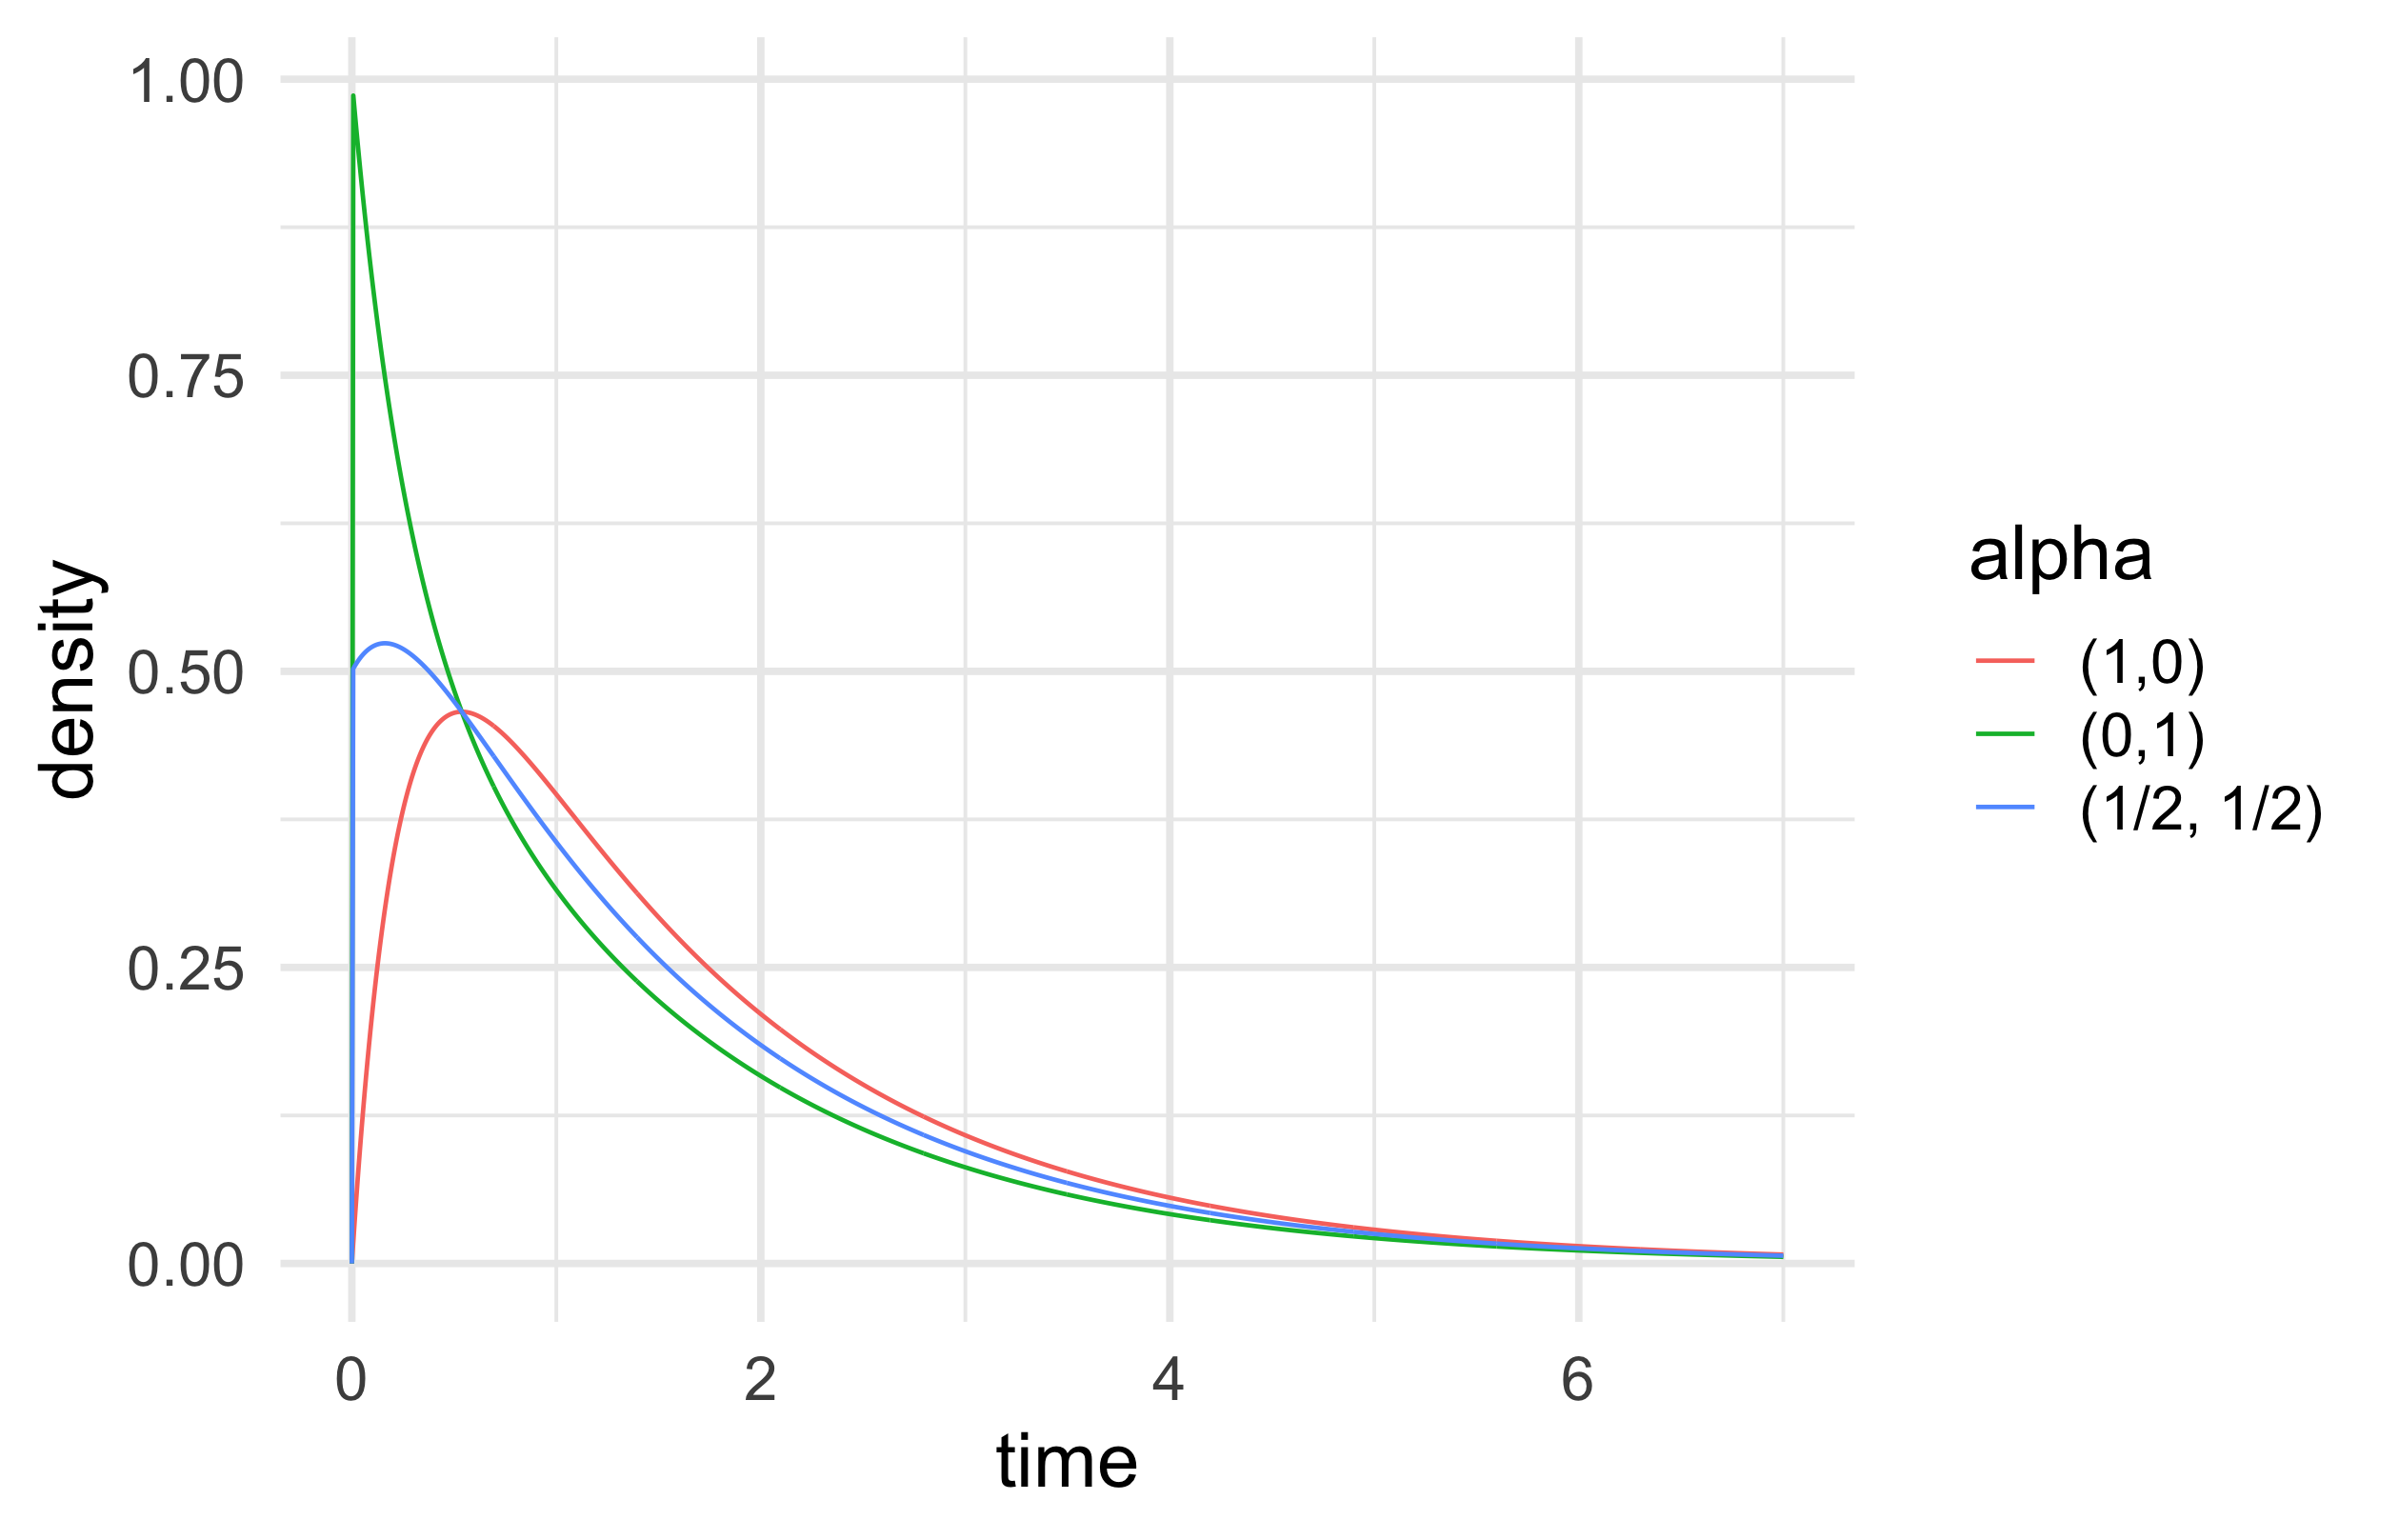
\includegraphics[width=.80\textwidth]{figures/voter_density_c4.png}
   \caption{Density of the absorption time for the voter model on the complete graph with four nodes, $C_4$. The initial stating position is varied between always stating at state $2$, starting at start $1$ and an equal mixture of starting at either 1 or 2.}
  \label{fig:voter_density_c4}
\end{figure}

\subsection{Complete voter model n nodes  \texorpdfstring{$C_n$}{VCn}}
If $n$ is even, then let $k = n / 2$ and if $n$ is odd then let $k = (n - 1)/2$.
We have $\{0,\ldots, k\}$ projected states.
Assume we are in state $i \not = k$.
To transition to state $i + 1$, we have $n - i$ nodes that can flip to match the $i$ nodes.
Each one of these nodes will flip with a rate of $\frac{i}{n - 1}$ since the graph is complete and each node is connected to $i$ nodes with the opposite rate.
Thus, the rate is $(n - i) \frac{i}{n - 1}$.
Similarly for $i \to i - 1$ transition we have $i$ nodes that can flip at a rate of $\frac{n - i}{n - 1}$ leading to the same rate.
If $i = k$, and $n$ is even, then we have all $n$ sites that can switch, each at a rate of $k / (n - 1)$.
If $i = k$, and $n$ is odd, then we have $k$ sites that can switch, each at a rate of $(n - k ) / (n - 1)$.
We can summarize the rates as follows:
\begin{align*}
    i \to i - 1 &= \begin{cases}
        0 & i = 0\\
        \frac{1}{n - 1} nk & i = k, n \text{ even}\\
        \frac{1}{n - 1}k (n - k) & i = k, n \text{ odd}\\
        \frac{1}{n - 1} i (n - i) & i \in \{1,\ldots, k - 1\}
    \end{cases}\\
    i \to i + 1 &= \begin{cases}
        0 & i \in \{0, k\}\\
        \frac{1}{n - 1} i (n - i) & i \in \{1,\ldots, k - 1\}
    \end{cases}
\end{align*}
The embedded discrete Markov chain is just a random walk on $\{0, k\}$ where 0 is absorbing and $k$ reflects back.

\begin{figure}[H]
  \centering
\begin{tikzpicture}[
   start chain = going right,
   -Triangle,
   every loop/.append style = {-Triangle}]
   \node[state, on chain]  (n) {k};
   \node[state, on chain]  (n1) {k - 1};
   \node[state, on chain]  (n2) {k - 2};
   \node[state without output/.append style={draw=none}, on chain]  (dots1) {...};
   \node[state, on chain]  (2) {2};
   \node[state, on chain]  (1) {1};
   \node[state, on chain]  (0) {0};

   \draw (n) edge[bend left] node[yshift=3mm]{$1$} (n1);
   \draw (n1) edge[bend left] node[yshift=-3mm]{$1/2$}(n);

   \draw (n1) edge[bend left] node[yshift=3mm]{$1/2$} (n2);
   \draw (n2) edge[bend left] node[yshift=-3mm]{$1/2$}(n1);

   \draw (n2) edge[left] node[xshift=3mm, yshift=-3mm]{} (dots1);

   \draw (dots1) edge[left] node[xshift=3mm, yshift=-3mm]{} (2);

  \draw (2) edge[bend left] node[yshift=3mm]{$1/2$} (1);
   \draw (1) edge[bend left] node[yshift=-3mm]{$1/2$}(2);

  \draw (1) edge[left] node[xshift=3mm, yshift=3mm]{$1/2$} (0);
\end{tikzpicture}
\caption{Embedded discrete Markov chain of the projected states of the $n$ node complete voter model.}
  \label{fig:rw_voter_model_discrete}
\end{figure}

\begin{lemma}\label{lem:rw_hit_zero}
Assume that we have a simple random walk on $\{0,1,\ldots, n\}$.
If we start in state $i \in \{1,\ldots, n - 1\}$, then the probability of hitting state 0 before state $k \in \{i + 1, \ldots, n\}$ is $\frac{k - i}{k}$.
\end{lemma}

\begin{proof}
Let $A_i$ be the probability of hitting state 0 before state $k$ when starting from state $i \in \{1,\ldots, n - 1\}$ which satisfies the recurrence relations
\begin{align*}
    A_0 &= 1\\
    A_{k} &= 0\\
    A_i &= \frac{1}{2} A_{i + 1} + \frac{1}{2} A_{i - 1}
\end{align*}

The characteristic equation is $f(x) = x^2 - 2x + 1$ which has a double root at $1$.
Thus the solution of is of the form $A_i = a + bi$ and using the boundary conditions of $A_0 = 1$ we get that $a = 1$, and $A_{k} = 0$ we get that $b = - 1/k$.
$$
A_i = \frac{k - i}{k}
$$
\end{proof}

\begin{theorem}
Assume that we have a simple random walk on $\{0,1,\ldots, k\}$ where 0 is absorbing and $k$ is reflecting as shown in Figure \ref{fig:rw_voter_model_discrete}.
Let $N_1, N_2, \ldots, N_k$ be the geometric random variables for the number of visits to each state.
Then,
$$
E[N_i] = \begin{cases}
    2i & 0 < i < k\\
    k & i = k
\end{cases}
$$
\end{theorem}

\begin{proof}
Using Lemma \ref{lem:rw_hit_zero} we have that for any $i \in \{1, \ldots, k - 1\}$ the probability of hitting 0 before hitting $i$ when at state $i - 1$ is $\frac{i - (i - 1)}{i} = \frac{1}{i}$.
Since we always return to $i$ if we move to $i + 1$, then the probability of never returning to $i$ is given by $\frac{1}{2i}$.
In the case when $i = k$, always go to the state $k - 1$ so the probability of never returning is simply $\frac{1}{k}$.
The result follows since the parameter in the geometric distribution is the probability of never returning to the state.
\end{proof}

\begin{defn}[Harmonic Number]
The $m$-th harmonic number defined as
$$
H_m = \sum_{j = 1}^m \frac{1}{j}
$$
Note that
$$
H_m = H_{m - 1} + \frac{1}{m}
$$
\end{defn}

\begin{theorem}\label{thm:euler_harm_lim}
$$
\lim_{n \to \infty} [H_n - \ln(n)] = \gamma
$$
where $\gamma \approx 0.5772$ is the Euler-Mascheroni constant.
\end{theorem}

\begin{theorem}
Let $\tau_{C_n}$ be the time until the voter model on the complete graph with $n$ nodes reaches $\equiv 1$ or $\equiv 0$.
Now let $N_1, N_2, \ldots, N_k$ be the number of visits to states $1, 2, \ldots, k$ respectively, which are geometrically distributed.
For all $i = 1,2,\ldots, N_i$ and $j = 1,2,\ldots, k$, let

$$
X_i^{(j)} \sim \begin{cases}
  \exp\left(\displaystyle \frac{nk}{n - 1}\right) & j = k, n \text{ even}\\[10pt]
  \exp\left(\displaystyle\frac{k (n - k)}{n - 1}\right) & j = k, n \text{ odd}\\[10pt]
  \exp\left(\displaystyle \frac{2j (n - j)}{n - 1}\right) & j \in \{1, \ldots, k-1\}
\end{cases}
$$
be i.i.d random variables representing the exponential waiting time at each state. Note that
$$
E[X_i^{(j)}] = E[X^{(j)}] = \begin{cases}
  \displaystyle \frac{n - 1}{nk} & j = k, n \text{ even}\\[10pt]
  \displaystyle \frac{n - 1}{k (n - k)} & j = k, n \text{ odd}\\[10pt]
  \displaystyle \frac{n - 1}{2j (n - j)} & j \in \{1,\ldots, k - 1\}\\
\end{cases}
$$

Assuming that we start in state $k$ we can represent $\tau_{C_n}$ as random sums
\begin{equation}\label{eq:wait_contact_sum_voter}
    \tau_{C_n} = \sum_{i = 1}^{N_k} X_i^{(k)} + \sum_{i = 1}^{N_{k - 1}} X_i^{(k - 1)} + \cdots + \sum_{i = 1}^{N_1} X_i^{(1)}
\end{equation}
and
\begin{align*}
E[\tau_{C_n}] &= \begin{cases}
    (n - 1) \left[H_{n} - H_{n - k}\right] & n \text{ even}\\
    (n - 1) \left[H_{n - 1} - H_{n - k - 1}\right] & n \text{ odd}
\end{cases}\\
\end{align*}
Also, $E[\tau_{C_n}]$ is approximately (denoted $\approx$) $\ln(2) (n - 1)$ for large $n$.
\end{theorem}

\begin{proof}
The random sums are not independent and have rather complicated dependencies but the expected value can be computed without independence.
Using Theorem \ref{thm:random_sum_ev}, the expected value of the random sums is
\begin{align*}
    E[\tau_{C_n}] &= E\left[\sum_{i = 1}^{N_k} X_i^{(k)} + \sum_{i = 1}^{N_{k - 1}} X_i^{(k - 1)} + \cdots + \sum_{i = 1}^{N_1} X_i^{(1)}\right]\\
    &= E[N_k] E[X^{(k)}] + E[N_{k - 1}] E[X^{(k - 1)}] + \cdots + E[N_1]E[X_i^{(1)}]\\
    &= E[N_k] E[X^{(k)}] + \sum_{j = 1}^{k - 1} E[N_j]E[X^{(j)}]\\
    &= k E[X^{(k)}] + \sum_{j = 1}^{k - 1} 2j \frac{n - 1}{2j (n - j)} \\
    &= k E[X^{(k)}] + (n - 1) \sum_{j = 1}^{k - 1} \frac{1}{n - j}\\
    &= k E[X^{(k)}] + (n - 1) \left[ \frac{1}{n - 1} + \frac{1}{n - 2} + \cdots + \frac{1}{n - k + 1} \right]\\
    &= k E[X^{(k)}] + (n - 1) \left[ H_{n - 1} - H_{n - k} \right]\\
    &= \begin{cases}
    (n - 1) \left[\frac{1}{n} + H_{n - 1} - H_{n - k}\right] & n \text{ even}\\
    (n - 1) \left[\frac{1}{n - k} + H_{n - 1} - H_{n - k}\right] & n \text{ odd}
    \end{cases}\\
    &= \begin{cases}
    (n - 1) \left[H_{n} - H_{n - k}\right] & n \text{ even}\\
    (n - 1) \left[H_{n - 1} - H_{n - k - 1}\right] & n \text{ odd}
\end{cases}
\end{align*}
In the limit, it does not matter if $n$ is even or odd.
We have from Theorem \ref{thm:euler_harm_lim} that
\begin{align*}
    \lim_{n \to \infty} [H_{n} - H_{n - k}] &=  \lim_{n \to \infty} [H_{n} - \gamma - (H_{n - k} - \gamma)]\\
    &= \lim_{n \to \infty} (\ln(n) - \ln(n/2))\\
    &= \ln(2) \approx 0.69
\end{align*}
Convergence is quite quick and at $n = 30$ we have that $|[H_{n} - H_{n - k}] - ln(2)| = 0.016$.
Therefore for large $n$ we can say that
$$
E[\tau_{C_n}] \approx \ln(2) (n - 1)
$$
\end{proof}

% \subsection{Four node cycle \texorpdfstring{$S_4$}{VS4}}
% State $2t$ is the configurations with the two matching values together such as $\{1100\}$ and $2s$ is the configuration with matching values apart such as $\{0101\}$

% \begin{figure}[H]
%     \centering
%   \begin{tikzpicture}[start chain = going right,
%   -Triangle, every loop/.append style = {-Triangle}]
%   \node[state, on chain]  (1) {1};
%   \node[state, on chain]  (2s) [left of=1, yshift = -10mm, xshift = -20mm]  {2s};

%   \node[state, on chain]  (2t) [left of=1, yshift = 10mm, xshift = -20mm]  {2t};

%   \node[state, on chain]  (0) [right of=1]  {0};

%     \draw (2t) edge [bend left] node[yshift=3mm, xshift=1mm]{$2$} (1);
%     \draw (1) edge [] node[yshift=-2mm, xshift=-1mm]{$1$} (2t);

%     \draw (2s) edge [] node[yshift=-3.5mm, xshift=1mm]{$4$} (1);

%     \draw (1) edge [] node[yshift=-2mm, xshift=-1mm]{$1$} (0);

% \end{tikzpicture}
%     \caption{Projected rates of the four node voter model on cycle. State $2t$ are the configurations with the two matching values together such as $\{1100\}$ and $2s$ are the configurations with matching values apart such as $\{0101\}$}
%     \label{fig:four_node_voter_cycle_rates}
% \end{figure}

% % Is it possible that we can use Burnside Polya counting (group actions) to show how many different distinct cycle configurations we get?

% \subsection{Torus in \texorpdfstring{$Z^d${Zd}}
